\section{Design of the template library}

\subsection{Task}
\label{section:interface}

In programming language, a function which can apply any values of
different types are parametric polymorphism. C++ has already supported
this language feature by template function. Our library needs to
manipulate template functions and instantiate them on demand, which we
call it \emph{late-instantiation} inspired of
\emph{late-binding}. Because the entry address of a template function is not available until instantiation, it is desirable to extend function
polymorphism for different template arguments  at compile-time. Our
approach is to wrap the template function by a template class and pass
it as \emph{template template class}. A wrapper function acts
as interface provided by algorithm developers. Fig.~\ref{lst:wrapper} is a wrapper function of vector addition. 

Beside it enables late-instantiation, the advantage of template class interface
is to provide different entries for different execution environments. \emph{doit\_b} is
used to implement synchronization in Fig.~\ref{fig:mm}.  Another benefit of
this form is that wrapper classes  give compiler a chance to select
appropriate codes based on their types, which is T in our example. This method incurs an extra function call  thought, it is hopefully  eliminated by
compiler's inline optimization.

\begin{figure}[!htp]
\begin{minipage}[tb]{\linewidth}
\makebox[\textwidth]{\hrulefill}
\begin{small}
\begin{verbatim}
/*A function wrapper for vector addition
 */
template<class Result, class Arg0, 
         class Arg1>
struct vecAddWrapper {
 //omitted...
 
 //entry
 static void 
 doit(const Arg0& arg0, const Arg1& arg1, 
     Result& result)
 {
  vecArithImpl<T, DIM_N>::add(arg0, arg1, 
                           result);
 }

 //entry with a barrier to synchronize
 static void 
 doit_b(const Arg0& arg0, const Arg1& arg1, 
     Result& result, mt::barrier& barrier)
 {
   doit(arg0, arg1, result);
   barrier.wait();
 }

 //...
};
\end{verbatim}
\end{small}
\makebox[\textwidth]{\hrulefill}
\end{minipage}
\caption{Function Wrapper}\label{lst:wrapper}
\end{figure}

\subsubsection{TF class}
%TF class
Computation-intensive functions are commonly referred to as
\emph{kernel} or \emph{filter}. Mathematically, a function is
single-target binary relation. Kernel functions are usually
self-contained, \textit{i.e.} external data references are limited and
calling graphs are simple. It's possible for a kernel function to
decouple into a cluster of subprocedures. Each subprocedure may be
exactly the same and spread on multicore to execute in
parallel.  Another approach is to divide a kernel into finer stages
and run in pipeline manner to respect data locality and memory bandwidth. In
libvina, a \emph{transform class (TF class)} is a template class which
transforms a function to a cluster of subprocedures in isomorphism. As
shown in Fig.~\ref{fig:tfcls}, the transformed function on right sisde
has the same interface while owns a call graph to complete the
original computation by a cluster of subprocedures. Execution of the
call graph can be programmed by in the library to take advantage of
architectural features.

\begin{figure}
\centering
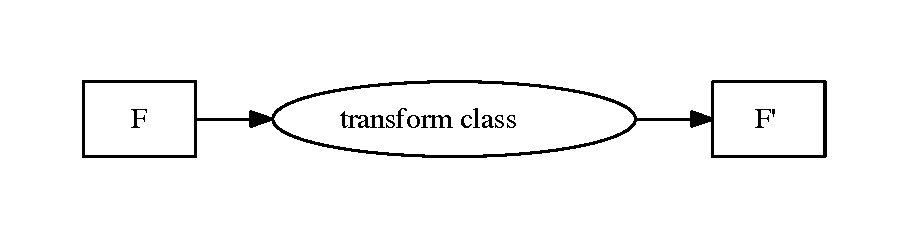
\includegraphics[width=3.1in]{map-class}
\caption{transform class}\label{fig:tfcls}
\end{figure}


%predicate and sentinel
\subsubsection{Predicate}
Borrowed from lisp concept, \emph{predicate} represents an indicator
of some conditions. It is a template class with static
fields initialized by constant expressions consisting of template
parameters and constants. These fields are automatically evaluated
when template classes are instantiated. Fig.~\ref{lst:pred} is an example to determine whether the problem size is fitting for last level cache.

\begin{figure}[!htp]
\begin{minipage}[tb]{\linewidth}
\makebox[\textwidth]{\hrulefill}
\begin{small}
\begin{verbatim}
/*determine whether the problem size is 
 *less than last level cache.
 */
template <class T, int SIZE_A
     , int SIZE_B, int SIZE_C>
struct p_lt_cache_ll {
 enum {CACHE_LL_SIZE = 4096*1024};
 const static bool value = 
     ((SIZE_A * SIZE_B 
   + SIZE_A * SIZE_C + SIZE_B * SIZE_C) 
   * sizeof(T) ) <= CACHE_LL_SIZE;
};
\end{verbatim}
\end{small}
\vspace{-1ex}\makebox[\textwidth]{\hrulefill}
\end{minipage}
\caption{Predicate}\label{lst:pred}
\end{figure}

\subsubsection{Sentinel}
\emph{Sentinels} in libvina are non-type template parameters of
\emph{TF class}. When a template class is instantiating, sentinels are
evaluated from a \emph{predicate}.  The \emph{predicate} determines
whether a specific requirement has been satisfied. Sentinel is
responsible for changing generation strategy according to the
result. Using \emph{template specialization}, C++ compiler chooses
different versions of class to instantiate basing on the values or
types of template arguments. The most important application of
\emph{sentinel} is to  terminate recursion. More general flow control
such as branch is available in MPL ~\cite{mpl}.

\subsection{Supporting data structures}
Template metaprograming works in compile-time. Therefore, problems we can solve must have rich static
information. Fortunately,  applications with this characteristic are
not uncommon in multimedia or digital processing fields, some of them 
even attract developers to implement them in hardware such as FPGA or DSP. To leverage
static information, data structures need to associate template
arguments with such information. Only vector and matrix are implemented in libvina,
because they cover many applications in the fields mentioned
previously. Users require more versatile data structures can also
resort to MPL.

A \emph{View} class is a concept to represent data set.
Fig. ~\ref{fig:view} depicts relationship of views in libvina. Concrete lines
represent implicit conversion in C++, while  dashed lines are explicit
function calls to complete conversion. Text in edges are constraints
when conversions perform. Shadow region is another thread space. The
only approach to communicate with other threads is through a special view
class named ViewMT.  

Modern multicore architectures emphasize on utilization of 
bandwidth and storage-on-chip, therefore we manipulate data in
bulk. Essentially, a view is an abstract of \emph{stream} and it
helps programmers build streaming computation. Underneath view
classes, we can perform specialization based on architectures. \textit{e.g}, it is not necessary to duplicate
data  on shared memory, or  we can raise asynchronous communication to memory
hide latency. In addition, a view class is type-safed. Programmers can get
compilation errors if programs have potential violations of date access rules. Early errors are particularly
important to prevent programmer from trapping into multi-threaded bugs.

\begin{figure}
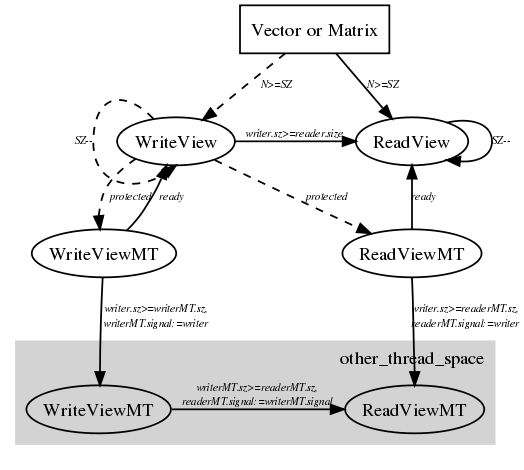
\includegraphics[width=3.3in]{../view_concept}
\caption{View classes in libvina}
\label{fig:view}
\end{figure}
%%
\section{Runtime supports}
Basically, our static transformation does not incur any runtime
overhead. However, we need thread and synchronization to execute in
multi-threaded environment.

We implemented \emph{mt::thread} based on underlying pthread. A
simple C++ thread pool is developed to reduce cost of thread
creation. Because pthread does not have group-scheduling, we design
and implement a lightweight thread library (libSPMD) based on Linux
clone(2) and semaphore. Other advantages of libSPMD
is that it provides hook function to perform reduction and CPU binding. 
On GPU, we use OpenCL ~\cite{opencl} to obtain platform
independence. Many accelerators are scheduled or declared to
implement OpenCL, which might extend our approach to new
territories in the future.  Although the interfaces of threads
mentioned before are varying, our library can deal with them well.

In libvina, we implement barrier for both CPU and GPU. CPU's
implementation uses pthread conditional variables, while GPU counterpart
uses openCL's API function. GPU's barrier synchronizes
\emph{work-groups}. We still can not find a good method to generate kernel
barrier statement worked on \emph{work-items}.

We define a signal class to synchronize, which mimic
signal primitive on CellBE~\cite{cellnetwork}. It is implemented by
conditional variable on x86. On GPU, we use \emph{event} of OpenCL to
achieve the same semantics.

